\section{Theoretical Framework} 

%----------------------------------------------------------------------------------------
% Equations slide
\begin{frame}{Equations}
\[
E=mc^2
\]
\begin{equation}
\hat{\beta} = 
\end{equation}
\end{frame}

% Double-Sided slide
\begin{frame}[allowframebreaks]{Double-Sided Slide}
This slide is split into multiple frames.
\framebreak
Second part of the slide.
\end{frame}

% Block slide
\begin{frame}{Block}
\begin{block}{Block Title}
This is a block.
\end{block}
\begin{alertblock}{Alert Block Title}
This is an alert block.
\end{alertblock}
\begin{exampleblock}{Example Block Title}
This is an example block.
\end{exampleblock}
\end{frame}

% Theorem slide
\begin{frame}
\begin{Theorem}
XYZ 
\end{Theorem}
\end{frame}

% Overlay slide
\begin{frame}{Overlay}
\begin{itemize}
\item<1-> Item 1
\item<2-> Item 2
\item<3-> Item 3
\end{itemize}
\end{frame}

% Image and Text slide
\begin{frame}{Image and Text}
\begin{columns}
\begin{column}{0.4 \textwidth}
\begin{figure}
\includegraphics[width=\textwidth]{example-image}
\caption{Caption}
\end{figure}
\end{column}
\begin{column}{0.4\textwidth}
Some text.
\end{column}
\end{columns}
\end{frame}

% Bullet Points slide
\begin{frame}{Bullet Points \& Enumerate}
\begin{itemize}
\item Bullet point 1
\item Bullet point 2
\item Bullet point 3
\end{itemize}
\begin{enumerate}
\item Bullet point 1
\item Bullet point 2
\item Bullet point 3
\end{enumerate}
\end{frame}

% Table slide
\begin{frame}{Table}
\begin{tabular}{|c|c|}
\hline
A & B \\
\hline
1 & 2 \\
3 & 4 \\
\hline
\end{tabular}
\end{frame}

% Top Centered Slide
\begin{frame}[t]{Top Centered Slide}
This slide is centered at the top.
\end{frame}

%E pochal Slide
\begin{frame}{Epochal Slide}
\centering
\textbf{\Huge Epochal Event}
\end{frame}

% Quote Slide
\begin{frame}{Quote Slide}
\begin{quote}
This is a quote.
\end{quote}
\end{frame}

% Code Slide
\begin{frame}[fragile]{Code Slide}
\begin{verbatim}
for i in range(5):
    print(i)
\end{verbatim}
\end{frame}

% Image Grid Slide
\begin{frame}
\frametitle{Image Grid Slide}
\begin{figure}
\includegraphics[width=0.3\textwidth]{example-image-a}
\includegraphics[width=0.3\textwidth]{example-image-b}
\includegraphics[width=0.3\textwidth]{example-image-c}
\caption{Images in a grid}
\end{figure}
\end{frame}

% Two Columns Slide with Divider
\begin{frame}[t]
\frametitle{Two Columns Slide with Divider}
\begin{columns}[T]
\column{0.46\textwidth}
\underline{\textbf{Column 1 Subhead}}
\begin{itemize}
\item Text
\item Text
\end{itemize}

\column{0.02\textwidth}
\centering
\rule{0.5pt}{4cm} % Vertical divider

\column{0.46\textwidth}
\underline{\textbf{Column 2 Subhead}}
\begin{itemize}
\item Text
\item Text
\end{itemize}
\end{columns}
\vfill
\begin{block}{Takeaway Box}
Text
\end{block}
\vfill
\end{frame}

\begin{frame}{Mathematisches Diagramm}
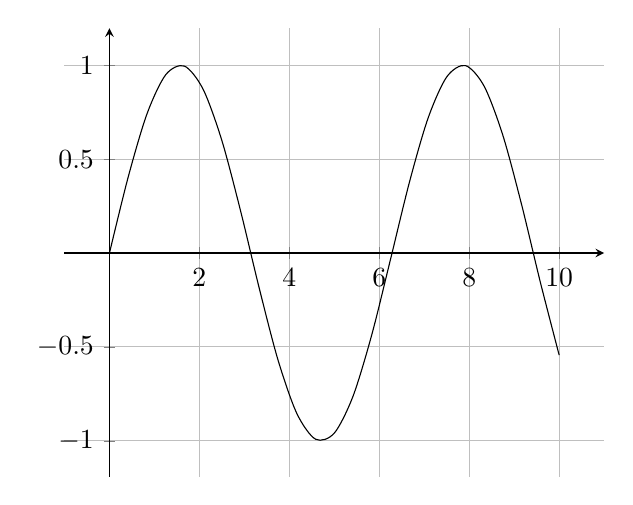
\begin{tikzpicture}
  \begin{axis}[
    axis lines = middle,
    enlargelimits = true,
    grid = major
  ]
  \addplot[smooth,domain=0:10] {sin(deg(x))};
  \end{axis}
\end{tikzpicture}
\end{frame}


\begin{frame}[fragile]{Code mit Syntax Highlighting}
\begin{stata}
capture drop newvar
generate newvar = oldvar * 2
\end{stata}
Der Befehl \statainline{generate newvar = oldvar * 2} erzeugt eine neue Variable.

\end{frame}

\begin{frame}{This paper in a nutshell I}
\vspace{-0.4cm}
\begin{table}[]
    \renewcommand{\arraystretch}{1.8} % Adjust line spacing in rows
    \setlength{\tabcolsep}{0.4em} % Adjust column spacing
    \centering
    \begin{tabular}{@{}clp{0.8\linewidth}@{}}
        \faQuestion & \textbf{Interest} & ``Intensive Margin'' of application effect, $\hat{\tau}$ \\[0.5cm]
        \faEdit & \textbf{Treatment} & Exploit quasi-experimental variation w.r.t. amount of SU klippers (2013 reform; Distance to graduation $\leq 2 \Rightarrow$ 12 klippers more $\uparrow$) \\[0.5cm]
        \faArrowsAltH &\textbf{Outcome} & $Y = \Pr(\text{HA}|\text{Application})$, whereas HA = Application to High Ambition Program  {\footnotesize \color{gray} (c.f. Almer et al. 2024)} \\[0.5cm]
        \faDatabase & \textbf{Data }& $\text{KOT} \cup \text{Register Data}$ \\
    \end{tabular}
\end{table}
\vfill
\end{frame}

\begin{frame}{This paper in a nutshell II }
\vfill
\hspace{0.2em} \faEdit \hspace{0.5em} \textit{Treatment:} Free tuition for high-achieving, low income students (ex-ante knowledge)
\vfill

\hspace{0.2em} \faArrowsAltH  \hspace{0.5em} \textit{Outcomes:} Application, admission, enrollment rates
\vfill
\hspace{0.2em} \faBriefcase \hspace{0.5em} \textit{Method:} RCT
\vfill
\hspace{0.2em} \faDatabase \hspace{0.5em} \textit{Data:} Administrative data from Michigan (longitudinal at student level)
\vfill
\hspace{0.2em} \faCheckCircle \hspace{0.5em} \textit{Findings:} Significant increase of application and enrollment rates for low income students
\vfill
\end{frame}


% You can add frame-1.pdf until frame-10.pdf and it animates it. Can change the numberrs accordingly.
% \begin{frame}{Animierte Bilder}
%  \animategraphics[autoplay,loop,scale=0.5]{10}{frame-}{1}{10}
% \end{frame}
